\section{Statement of the problem}

Considering a plant with switched-affine dynamics described by: 

\noindent
\begin{equation}
    \label{eq:cap4:continuous-time-dynamics}
    \dot{x}(t) = A_{\sigma(t)} x(t) + b_{\sigma(t)}
\end{equation}


We assume the existence of a periodic switching signal \highlight{$\bar{\sigma}(t)$}
associated with a periodic trajectory \highlight{$\bar{x}(t)$}, as obtained in 
Chapter \ref{chap:cap2:target-periodic-trajectories}. Our objective is to introduce perturbations 
in the switching instants such that the trajectory \highlight{$x(t)$} converges to the reference trajectory \highlight{$\bar{x}(t)$}.

\begin{figure}[h]
    \centering
    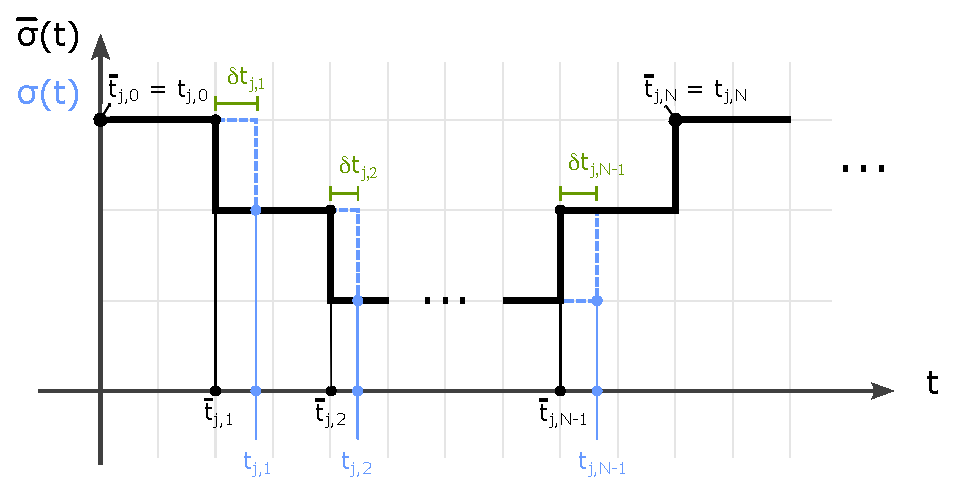
\includegraphics[]{figures/cap4/desenho_cap4_3.eps}
    \caption{Switching signals}\label{fig:cap4:switching-signals}
\end{figure}


Figure \ref{fig:cap4:switching-signals} displays the \highlight{$j$th} cycle of the switching signals \highlight{$\bar{\sigma}(t)$} and \highlight{$\sigma(t)$},
which comprise \highlight{$N$} switching actions. Within this cycle, the \highlight{$i_{th}$} switching times of \highlight{$\bar{\sigma}(t)$} and 
\highlight{$\sigma(t)$} are denoted by \highlight{$\bar{t}_{j, i}$} and \highlight{$t_{j, i}$}, respectively.
The relation between \highlight{$\bar{t}_{j, i}$} and \highlight{$t_{j, i}$} is given by

\noindent
\begin{equation}
    t_{j, i} = \bar{t}_{j, i} + \delta t_{j, i}
\end{equation}

In what follows, we derive a linear equation that relates the 
switching times and the resulting deviation of \highlight{$x(t)$} with respect to \highlight{$\hat{x}(t)$} at the end of one cycle.
In the development of this linearization procedure, the \highlight{$j$} index will be dropped for brevity and simpler notation.